\documentclass{beamer}

\usepackage[utf8]{inputenc}
\usepackage[T1]{fontenc}
\usepackage{lmodern}
\usepackage{color}
\usepackage{fix-cm}
\usepackage{textpos}
\usepackage{eurosym}
\usepackage{multirow}
\usepackage{perpage}

% Redéfinis les marges des tableaux
\let\oldtabular=\tabular
\def\tabular{\small\oldtabular}
\renewcommand{\arraystretch}{1.5}

\usetheme{Warsaw}
\usecolortheme{orchid}

% Permet de réinitialiser les footnote à chaque frame. Nécéssite 2 compilations.
\MakePerPage{footnote}

\setlength{\TPHorizModule}{0.01\textwidth}
\setlength{\TPVertModule}{0.01\textheight}

\setbeamertemplate{navigation symbols}{}

\title[D.E.I - Gittip]{Gittip et le financement de l'open source.}
\author[J.AUTRAN \and FX.BELIGAT \and B.HOUDAYER \and A.RUHIER]{
	Jeremy AUTRAN\\
    \and
    François-Xavier BELIGAT\\
    \and
    Benoit HOUDAYER\\
	\and
	Anthony RUHIER
}
\institute[D.E.I]{D.E.I\\\ \\IUT Belfort Montbéliard}
\date{13 novembre 2013}

\begin{document}

% Permet de masquer le comptage de slides
\bgroup
\makeatletter
\setbeamertemplate{headline}{}
\setbeamertemplate{footline}
{
  \leavevmode%
  \hbox{%
  \begin{beamercolorbox}[wd=.5\paperwidth,ht=2.25ex,dp=1ex,center]{title in head/foot}%
    \usebeamerfont{title in head/foot}\insertshorttitle
  \end{beamercolorbox}%
  \begin{beamercolorbox}[wd=.5\paperwidth,ht=2.25ex,dp=1ex,center]{date in head/foot}%
    \usebeamerfont{date in head/foot}\insertshortdate{}
%    \insertframenumber{} / \inserttotalframenumber\hspace*{2ex}
  \end{beamercolorbox}}%
  \vskip0pt%
}
\makeatother

\begin{frame}[noframenumbering]
 	\frametitle{}
	\titlepage
\end{frame}
\egroup

\begin{frame}[plain]
	\begin{textblock}{0}(5,-30)
        \center{
\includegraphics[width=.7\paperwidth]{images/gittip.eps}}
	\end{textblock}
\end{frame}

\logo{\includegraphics[height=1cm]{images/logo-iut.eps}}


% Ajout du compteur de slides
\expandafter\def\expandafter\insertshorttitle\expandafter{%
      \insertshorttitle\hfill%
      \insertframenumber\,/\,\inserttotalframenumber}

\setcounter{framenumber}{0}

\begin{frame}
	\begin{small}
	\frametitle{Sommaire}
	\tableofcontents
	\end{small}
\end{frame}

\AtBeginSection[]
{
	\begin{small}
	\begin{frame}
		\frametitle{Sommaire}
		\tableofcontents[currentsection]
	\end{frame}
	\end{small}
}


%%%% Includes des sections :
%%%%%%%%%%%%%%%%%%%%%%%%%%%%%%
%
    \section{Présentation de Gittip}


\begin{frame}
\begin{itemize}
    \itemsep1.5em
    \item Système open source de micro-dons réguliers
    \item Dons hebdomadaires (chaque mardi)
    \item Créé le 11 mai 2012 par \textbf{Chad Whitacre}
    \item Novembre 2013 :
        \begin{itemize}
            \item \textbf{22 000} utilisateurs, dont \textbf{2 000} actifs.
            \item \textbf{7 300\${}} au total transférés chaque semaine
        \end{itemize}
\end{itemize}
\end{frame}


    \subsection{Un système de micro-dons libre}


{
\logo{}
\begin{frame}
\frametitle{Aspects communautaires}
\begin{center}
\begin{columns}
\begin{column}{260px}
{
    \begin{figure}[h!]
        \centering
        
\includegraphics[width=240px]{images/section1/homepage-gittip.eps}
        \caption{Page d'accueil de gittip.com}
    \end{figure}
}
\end{column}
\end{columns}
\end{center}
\end{frame}
}


{
\logo{}
\begin{frame}
\begin{center}
\begin{columns}
\begin{column}{260px}
{
    \begin{figure}[h!]
        \centering
        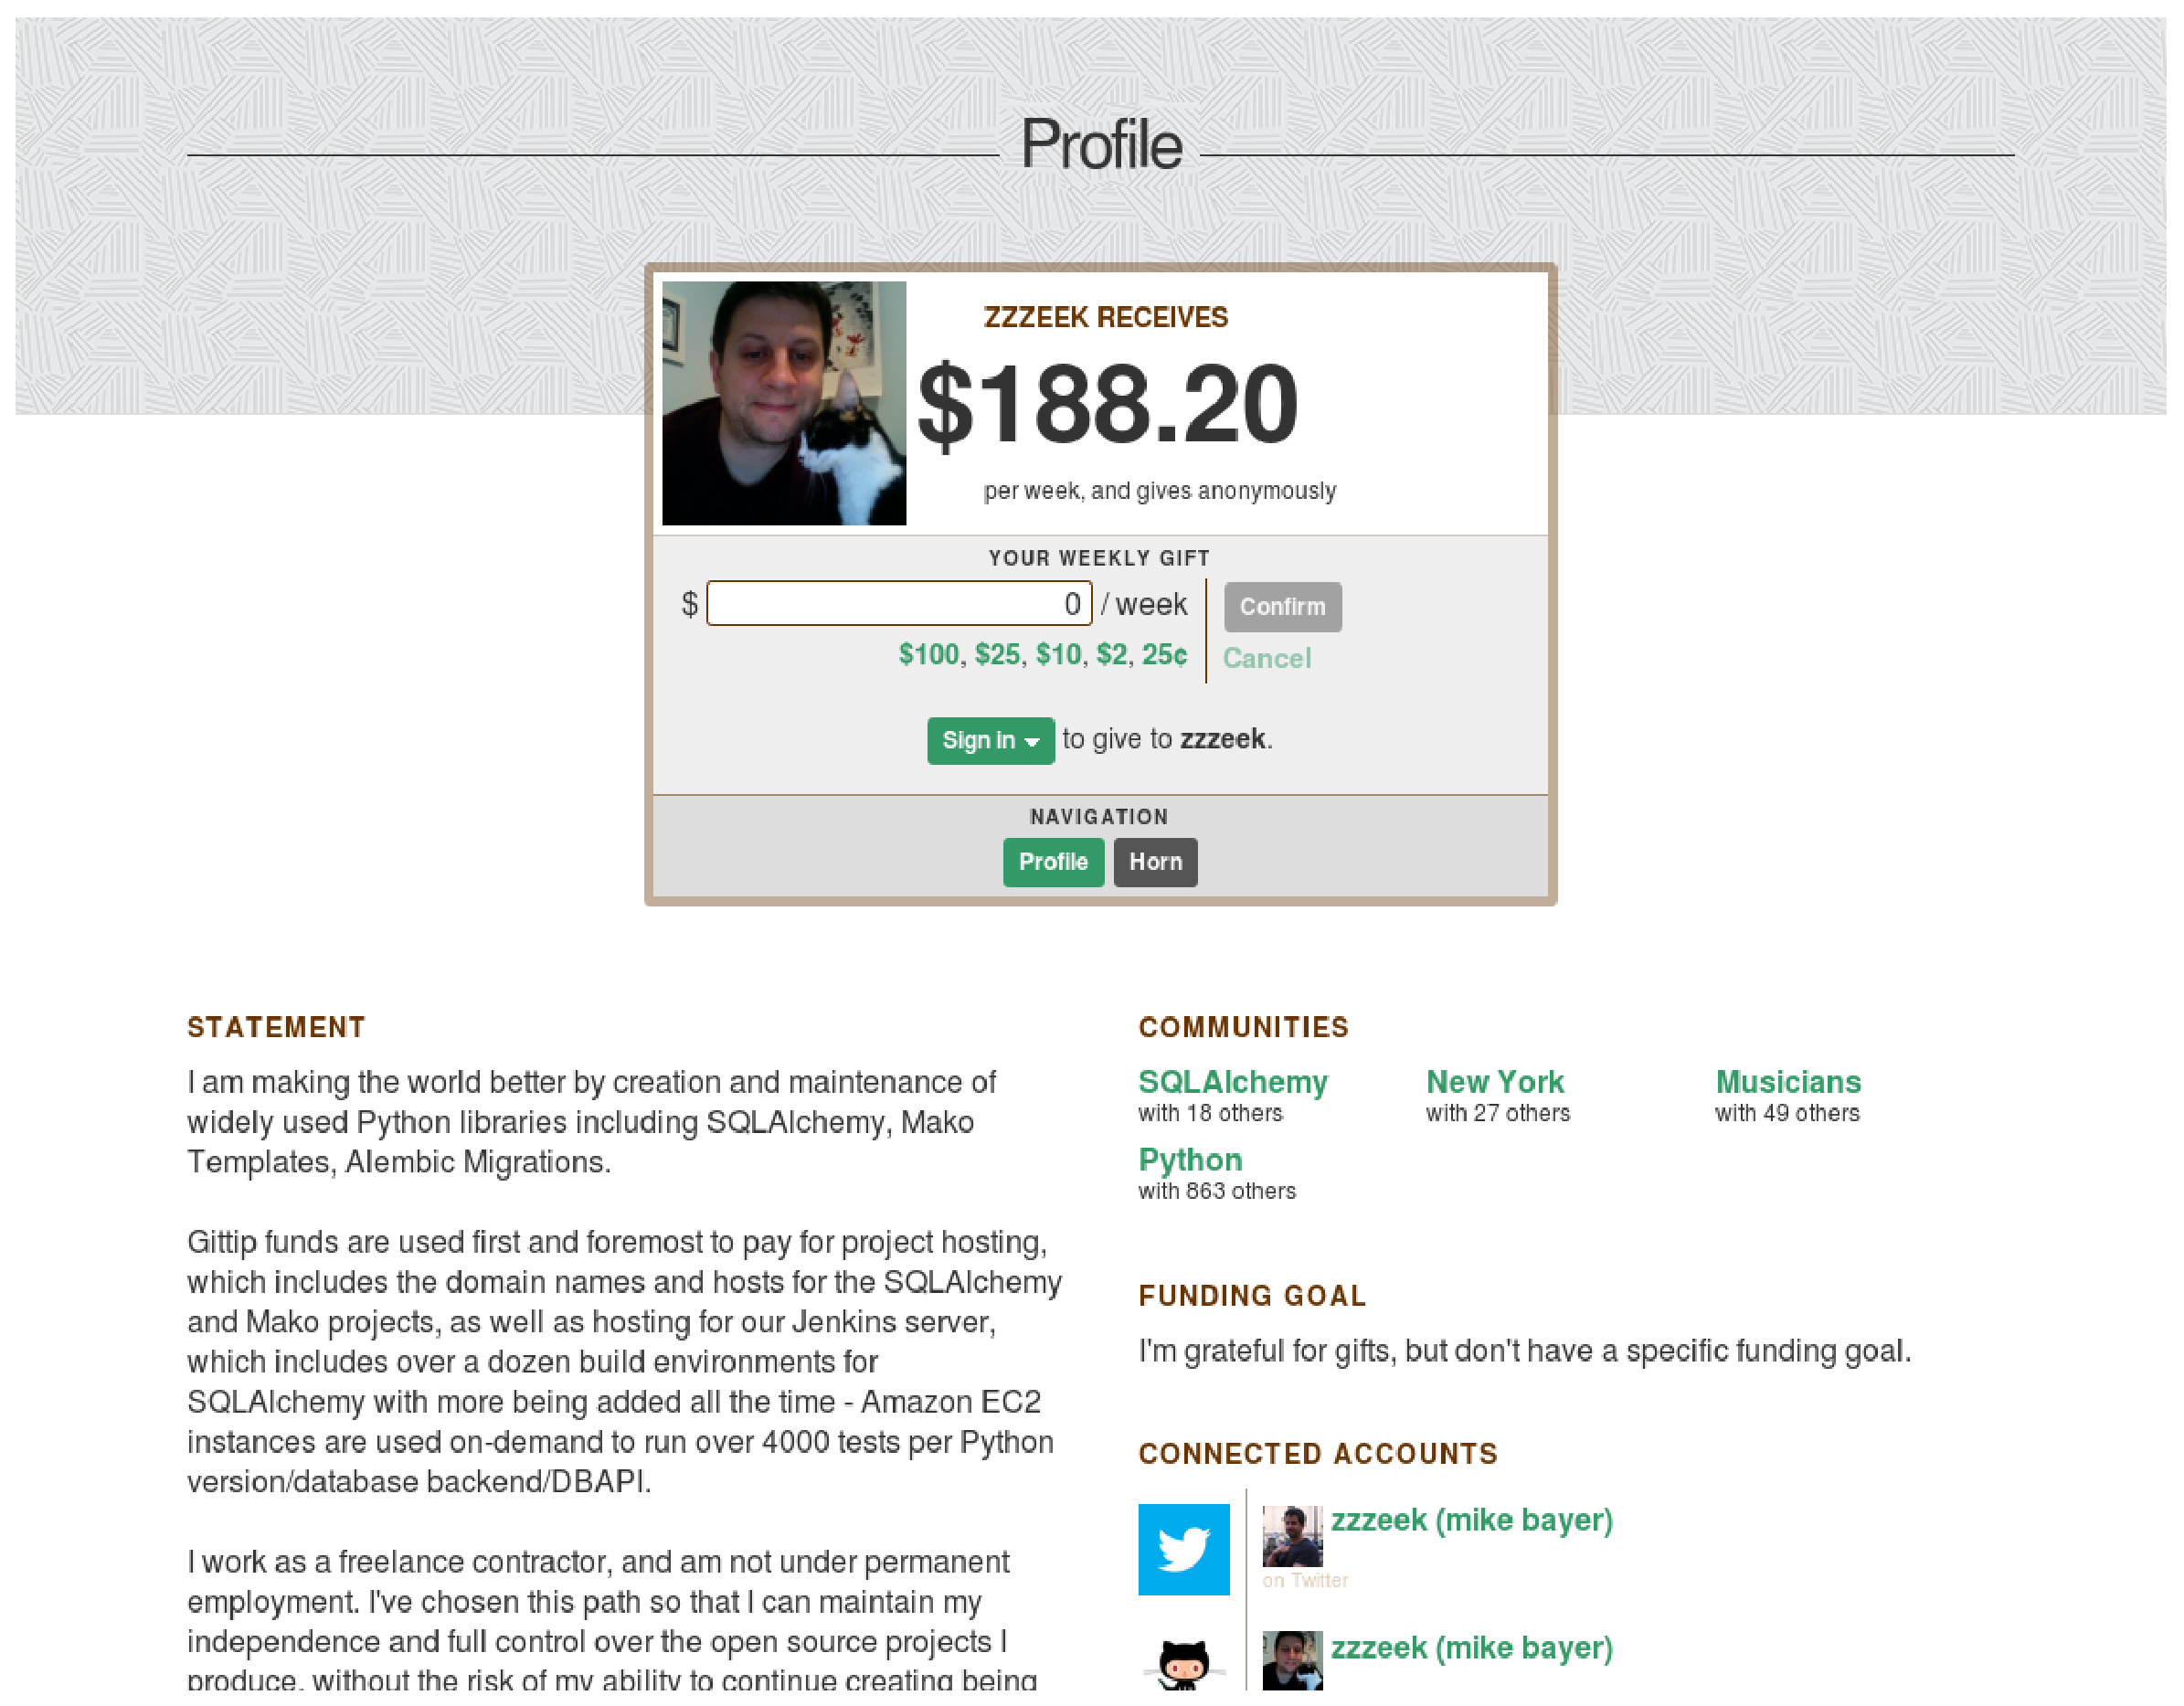
\includegraphics[width=240px]{images/section1/profilepage-gittip.eps}
        \caption{Exemple d'une page de profil sur gittip.com}
    \end{figure}
}
\end{column}
\end{columns}
\end{center}
\end{frame}
}


\begin{frame}

\begin{itemize}
    \itemsep1.5em
    \item Équipes de 150 personnes maximum (nombre de Dunbar)
    \item Communautés d'au moins 150 personnes
    \item ``Kids eat first''
    \item Basé sur l'individu
\end{itemize}
\end{frame}

    \subsection{L'open company Gittip LLC}


\begin{frame}
\frametitle{L'open company \emph{Gittip LLC}}

\begin{itemize}
    \itemsep1.5em
    \item Créée en février 2012 par Chad Whitacre
    \item 2ème open company
    \item 176 employés en novembre 2013
    \item Basée sur la transparence
    \item Sans hiérarchie
\end{itemize}
\end{frame}


\begin{frame}
\frametitle{Le type d'open company}

\begin{itemize}
    \itemsep1.5em
    \item Inventé en mars 2009 par Alexander Stigsen
    \item Basée sur la confiance
    \item Trust Metric
\end{itemize}
\end{frame}


    \section{Les autres modèles de financement}

\begin{frame}
\frametitle{Dons}

\begin{itemize}
    \itemsep1.5em
    \item Majoritairement via Paypal
    \item Peu de visibilité
    \item Manque de transparence
    \item Récurrence non prévue
\end{itemize}
\end{frame}


\begin{frame}
\frametitle{OpenBSD}

\begin{itemize}
    \itemsep1.5em
    \item Proche du don
    \item Plus d'intérêt à donner
\end{itemize}
\end{frame}

    \subsection{Modèles business friendly}

\begin{frame}
\frametitle{Licence double}

\begin{itemize}
    \itemsep1.5em
    \item Utilisé par MySQL
    \item Stratégie augmentant la visibilité
    \item Facilite la conversion de clients.
\end{itemize}
\end{frame}


\begin{frame}   % Anthony
\frametitle{Modèle Redhat}

\begin{itemize}
    \itemsep1.5em
    \item Monétisation sur les services périphériques
    \item Modèle le plus business friendly
    \item C.A de Redhat en 2012 : 1 milliards \${}
\end{itemize}
\end{frame}


\begin{frame}
\frametitle{Modèle Owncloud}

\begin{itemize}
    \itemsep1.5em
    \item Proche du modèle Redhat
    \item Vente de produit associé
\end{itemize}
\end{frame}


    \subsection{Modèles d'avant garde}


\begin{frame}
\frametitle{Modèle Bounty}

\begin{itemize}
    \itemsep1.5em
    \item Bonne visibilité
    \item Accent sur les fonctionnalités
\end{itemize}
\end{frame}


\begin{frame}
\frametitle{Pay What You Want}

\begin{itemize}
    \itemsep1.5em
    \item Peu développé pour l'open source
    \item Utilisé par Subsonic
    \item Principe du Humble Bundle
    \item Forte visibilité
\end{itemize}
\end{frame}


\begin{frame}
\begin{center}
\begin{columns}
\begin{column}{330px}
{
    \begin{figure}[h!]
        \centering
        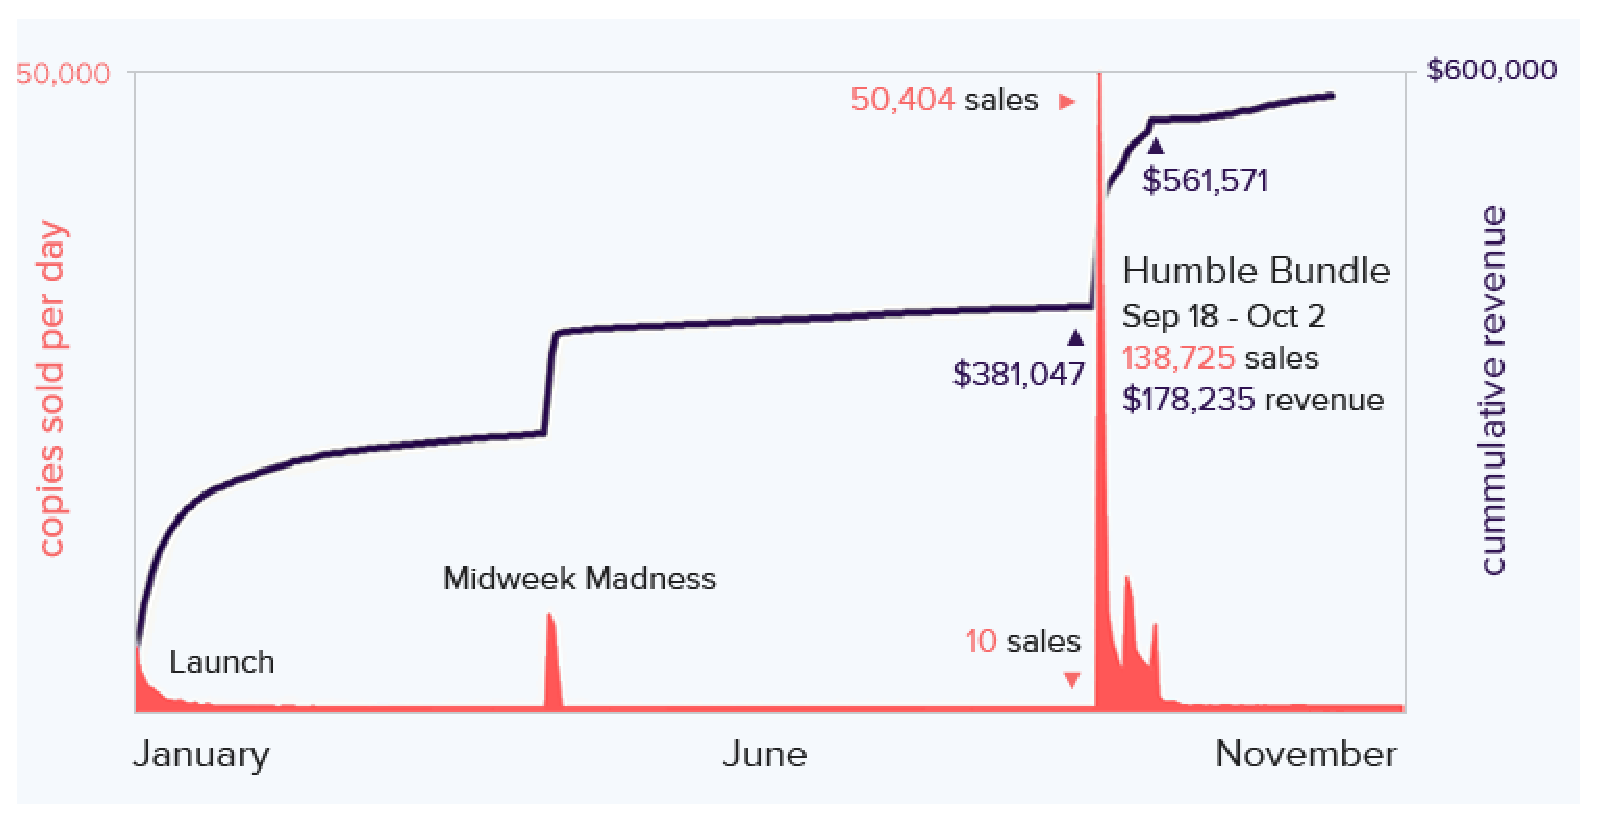
\includegraphics[width=310px]
            {images/section1/courbe-ventes-dustforce.eps}
        \caption{Évolution des ventes et des revenus du jeu Dustforce}
        \scriptsize{Source :
            \url{http://hitboxteam.com/dustforce-sales-figures}}
    \end{figure}
}
\end{column}
\end{columns}
\end{center}
\end{frame}


\begin{frame}   % Anthony
\frametitle{Crowdfounding}

\begin{itemize}
    \itemsep1.5em
    \item Permet le lancement de projet
    \item Forte visibilité
    \item Amène à la méritocratie
    \item Permet de grosses entrées d'argent
\end{itemize}
\end{frame}


\begin{frame}
\frametitle{Micro-paiement (flattr)}

\begin{itemize}
    \itemsep1.5em
    \item Principalement utilisé par les blogueurs
    \item ``Pay per like''
    \item Récurrence facilitée mais pas automatique
\end{itemize}
\end{frame}


\begin{frame}
\frametitle{Modèle Apple}

\begin{itemize}
    \itemsep1.5em
    \item Efficace
    \item Éthique douteuse
\end{itemize}
\end{frame}


    \section{Fiscalité}

    \subsection{Acteurs}


\begin{frame}
\frametitle{Acteurs}

\begin{itemize}
    \itemsep1.5em
    \item Donateur
    \item Donataire
    \item Intermédiaire
    \item Fisc, I.R.S
    \item \textbf{I.R.S :} Internal Revenue Service
\end{itemize}
\end{frame}


    \subsection{Aux États-Unis}

\begin{frame}
\frametitle{Aux États-Unis}

\begin{itemize}
    \itemsep1.5em
    \item Culture du don
    \item Abattement fixé à 13 000\${} en 2012
    \item Donateur imposable
\end{itemize}
\end{frame}


    \subsection{En France}


\begin{frame}
\frametitle{Catégories de dons}

\begin{itemize}
    \itemsep1.5em
    \item Les présents d'usage
    \item Les donations
\end{itemize}
\end{frame}


\begin{frame}
\frametitle{Le revenu}

\begin{itemize}
    \itemsep1.5em
    \item Salaire
    \item \textbf{BIC :} Bénéfices industriels et commerciaux
    \item \textbf{BNC :} Bénéfices non commerciaux
\end{itemize}
\end{frame}


    \section{Conclusion}


\begin{frame}
\frametitle{Conclusion}
\begin{itemize}
    \itemsep1.5em
    \item Novateur et intéressant
    \item Pas suffisamment développé
    \item Peu pratique en France
\end{itemize}
\end{frame}

%\include{sections/section2}
%\include{sections/section3}
%\include{sections/section4}

\end{document}
